% Created 2021-07-21 qua 11:02
% Intended LaTeX compiler: pdflatex
\documentclass[11pt]{article}
\usepackage[utf8]{inputenc}
\usepackage[T1]{fontenc}
\usepackage{graphicx}
\usepackage{grffile}
\usepackage{longtable}
\usepackage{wrapfig}
\usepackage{rotating}
\usepackage[normalem]{ulem}
\usepackage{amsmath}
\usepackage{textcomp}
\usepackage{amssymb}
\usepackage{capt-of}
\usepackage{hyperref}
\author{Ruan Flaneto Cartier}
\date{\today}
\title{Projeto automação residencial}
\hypersetup{
 pdfauthor={Ruan Flaneto Cartier},
 pdftitle={Projeto automação residencial},
 pdfkeywords={},
 pdfsubject={},
 pdfcreator={Emacs 28.0.50 (Org mode 9.5)}, 
 pdflang={English}}
\begin{document}

\maketitle
\tableofcontents


\section{Resumo}
\label{sec:orgb775871}
Um projeto de automação residencial foi demandado. Para a minha casa, pretende-se usar os ESP8266 para cada tomada para poder ter conexão com o computador central (raspberry pi).
Eu vou me limitar ao backend senão o projeto vai ficar complicado demais.

\section{Lâmpadas}
\label{sec:org6092d4b}
\subsection{Descrição do circuito}
\label{sec:org9361b58}
Um pequeno trafo recebe a energia da tomada, é retificada por uma ponte retificadora e então o módulo relé com o esp8266 controla o chaveamento da lâmpada. Não menos importante, o interruptor da tomada dever ser alimentado por um resistor, cujo estado é lido por uma porta digital. Quase esqueci dos sensores de presença. Devido ao espaço ocupado, novos interruptores devem ser comprados.
Sendo assim, o \(\mu C\) precisará de 3 portas digitais para controlar os periféricos e mais talvez duas para poder programar em ISP.
Pretendo não fazer placa de circuito impresso para simplificar o projeto e tb no momento é impossível para mim imprimir sem uma impressora adequada.
\subsection{Componentes utilizados (por lâmpada)}
\label{sec:orgee139f4}
\begin{itemize}
\item[{$\boxtimes$}] 1 Trafo de carregador;
\item[{$\boxtimes$}] 4 Diodos 1n4007;
\item[{$\boxtimes$}] 1 Capacitor eletrolítico (47uF);
\item[{$\boxtimes$}] 1 Capacitor cerâmico (100nF);
\item[{$\boxtimes$}] 1 Sensor piroelétrico
\item[{$\square$}] 1 Conjunto de interruptor; (Precisa comprar)
\item[{$\boxtimes$}] 1 Módulo de acionamento de relé por ESP8266 (figura \ref{fig:module_esp01})
\end{itemize}
\begin{figure}[h!]
\caption{\label{fig:module_esp01}Módulo relé com ESP01 utilizado}
\centering
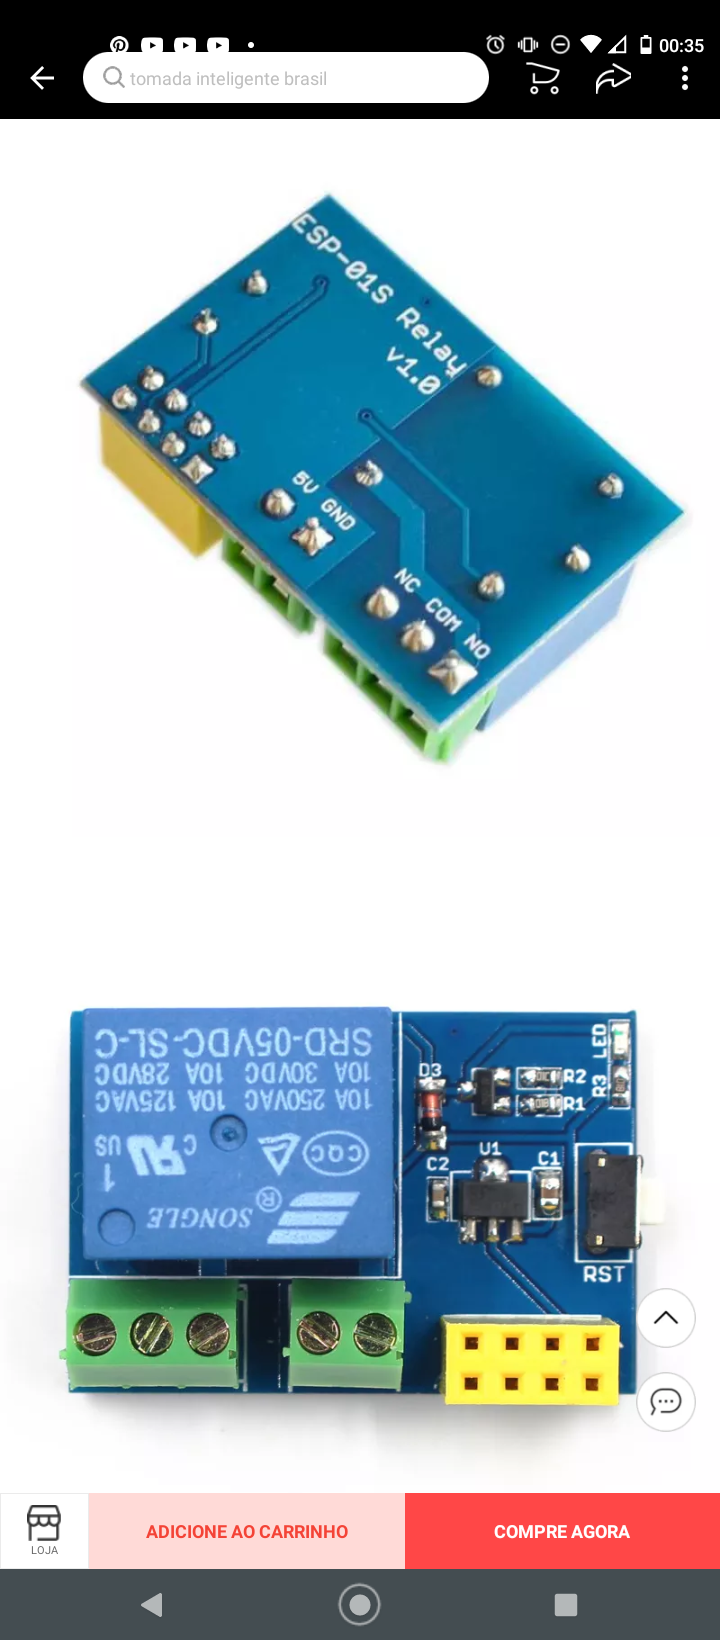
\includegraphics[width=0.3\textwidth]{./module_esp01.png}
\end{figure}

O módulo de relé possui o esquemático como na figura \ref{schematic_relay}
\begin{figure}[h!]
\caption{\label{fig:schematic_relay}Esquema do circuito do módulo com relé}
\centering
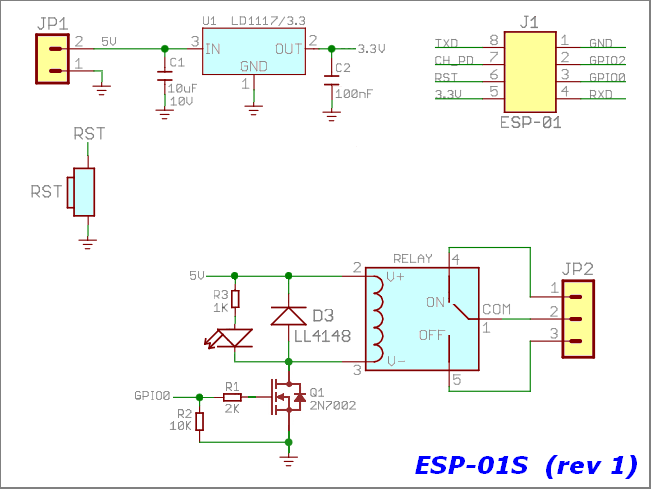
\includegraphics[width=0.3\textwidth]{./schematic_relay.png}
\end{figure}
\section{Controle do ar condicionado}
\label{sec:orgd5c48c9}
\subsection{Descrição do hardware}
\label{sec:orgb3ef852}
O computador principal se conecta ao controle do ar condicionado através dos barramentos de I2C do display e do microcontrolador. O primeiro barramento seria usado para o computador central identificar as configurações atuais do ar condicionado e o segundo serve para fazer alterações nas configurações. Para tanto é preciso fazer uma revisão sobre o protocolo e interpretar os dados lidos.
\subsection{I2C revisão}
\label{sec:org2aee7c8}
Ao abrir o controle do ar condicionado foram encontrados os pinos 36,37,38 e 44 acessíveis ao usuário. Como mostrado na figura \ref{fig:i2c_sh77}. Claramente eles servem para estabelecer comunicação i2c entre o chip e um computador externo.
\begin{figure}[h!]
\caption{\label{fig:i2c_sh77}Pinos i2c disponíveis ao usuário.}
\centering
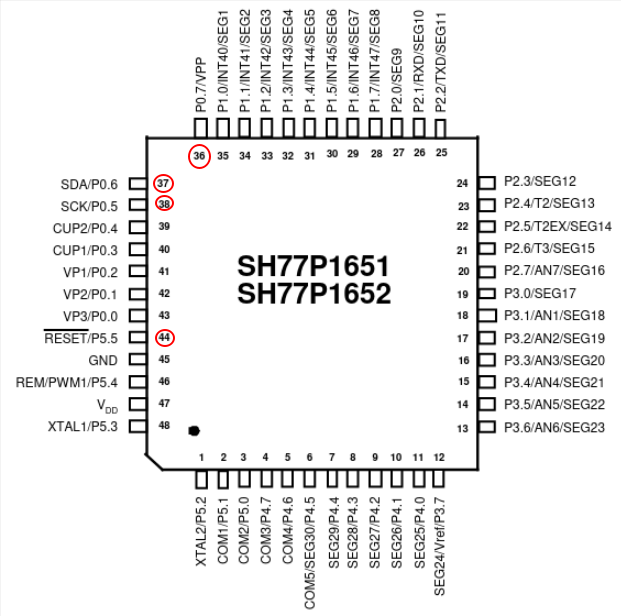
\includegraphics[width=0.6\textwidth]{./i2c_sh77.png}
\end{figure}

Fui procurar circuitos de controle remoto que aplicam este microcontrolador e achei um resultado interessante, como na figura \ref{fig:sh77_example}.

\begin{figure}[h!]
\caption{\label{fig:sh77_example}Pinos i2c disponíveis ao usuário.}
\centering
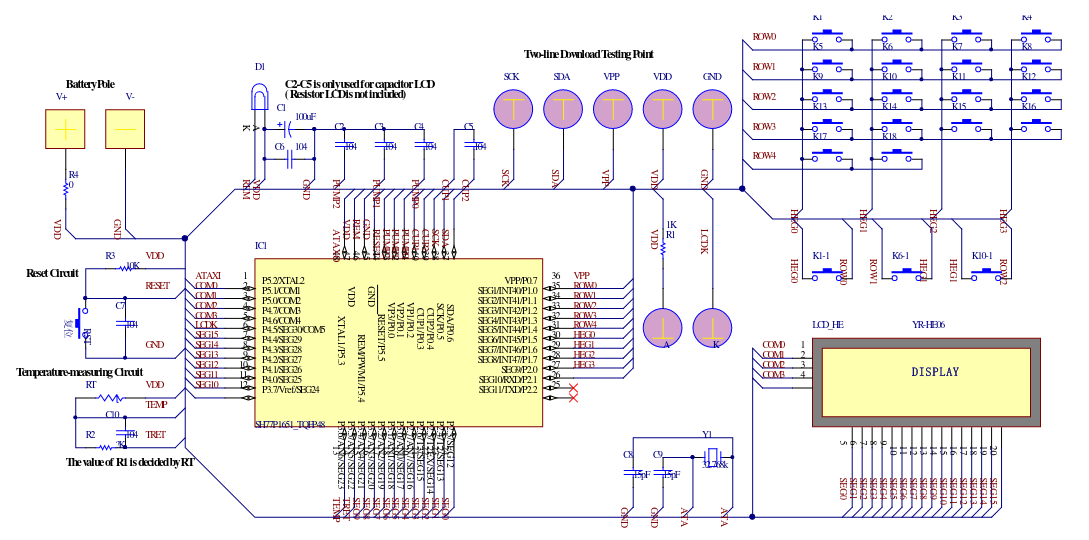
\includegraphics[width=0.6\textwidth]{./sh77_example.png}
\end{figure}

Logo fiquei na dúvida o que seria o VPP do pino 36, pesquisei no datasheet e achei este resultado (vide figura \ref{fig:vpp_meaning}).

\begin{figure}[h!]
\caption{\label{fig:vpp_meaning}Pinos i2c disponíveis ao usuário.}
\centering
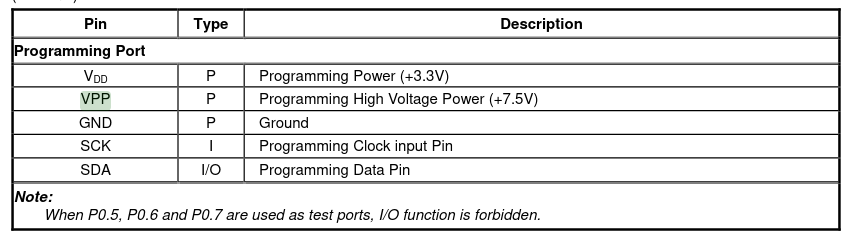
\includegraphics[width=0.6\textwidth]{./vpp_meaning.png}
\end{figure}

Depois disso notei que precisava rever um pouco sobre i2c e achei as seguintes figuras chave:
TODO \ldots{}


\section{Descrição do software}
\label{sec:orgf05a8fb}
Os esp8266 das tomadas devem entrar em um ponto de acesso central e então ficar à espera de comandos. Ele age como servidor para responder aos comandos do computador central, porém também irá enviar mensagens durante a comutação do sensor piroelétrico (descobrir se não vai haver realimentação positiva com a lâmpada)
Protocolo de comunicação:
Tem que descobrir uma forma de protocolar as mensagens. O receptor vai ler a mensagem e vai decodificá-la. Após decodificar, vai executar a ação de desligar/ligar.

USE o micropython, nada de C, para facilitar sua vida.

Procedimentos a serem utilizados na cpu principal:
\begin{itemize}
\item get state() \# Retorna o estado atual lâmpada;
\item get switch() \# Retorna a posição do interruptor;
\item turn(boolean state) \# Pede para ligar/desligar a lâmpada
\end{itemize}
\end{document}
